\documentclass[12pt,twoside]{article}
\usepackage{geometry}
\usepackage[shortlabels]{enumitem}
\setlist{nosep}
\setlist[enumerate]{wide=0pt, widest=99,leftmargin=25pt, labelsep=*}
\usepackage[none]{hyphenat}
\usepackage{graphicx}
\graphicspath{ {./} }
\usepackage{titlesec}
\usepackage{booktabs}
\usepackage{mathptmx}
\usepackage{setspace}
% --- Global paragraph formatting ---
\setlength{\parindent}{0pt}    % Removes first-line indentation
\setlength{\parskip}{1em}      % Adds space between paragraphs

\sloppy
\usepackage{array}
\newcolumntype{P}[1]{>{\centering\arraybackslash}p{#1}}
\newcolumntype{M}[1]{>{\centering\arraybackslash}m{#1}}


% --- Section title formatting ---
\titleformat{\section}
  {\normalfont\fontsize{12}{12}\bfseries}{\thesection.}{12pt}{}
\titlespacing*{\section}
  {0pt}{12pt plus 2pt minus 2pt}{0pt} % left, before, after

\titleformat{\subsection}
  {\normalfont\fontsize{12}{12}\bfseries}{\thesubsection}{12pt}{}
\titlespacing*{\subsection}
  {0pt}{10pt plus 2pt minus 2pt}{0pt}

\geometry{
 a4paper,
 total={170mm,257mm},
 left=2.54 cm,
 top=2.65 cm,
 right=2.54 cm,
 bottom=2.65 cm,
 }
 
 \rmfamily
\usepackage{fancyhdr}

\renewcommand{\footrulewidth}{0 pt}
\renewcommand{\headrulewidth}{0 pt}

\begin{document}

 \begin{singlespace}
 \begin{center}
\fontsize{24}{24}\selectfont\textbf
{Title of the Paper}
\end{center}
\vspace{24pt}
\fontsize{16}{16}\selectfont\textbf{
Author Name$^1$, Author Name$^2$}
\vspace{16pt}\\
\fontsize{11}{11}\selectfont {
$^1$Department, College, University, City, Country \\
$^2$Department, College, University, City, Country
}\vspace{16pt}\\
{\fontsize{9}{9}\selectfont\textbf{{E-mail:}} $^1$author1@college.edu, $^2$author2@institute.com}\\

\end{singlespace}
\fontsize{12}{12}\selectfont
\begin{onehalfspace}
\section*{Abstract}
Abstract goes here. 

\vspace{5pt}\\
\textbf{\fontsize{12}{12}\selectfont Keywords:} Keywords go here

\section{{Introduction}}
{Content goes here}
\vspace{10pt}
\subsection{Sub Heading}
{Content goes here}
\vspace{10pt}
\section{Related Work}
{Content goes here}\\
\\
{Cite the reference sequentially.  For example: Author et.al [1] or XYZ technique [2]}
\vspace{10pt}

\begin{center}
\textbf{Table 1.} Example table\\\vspace{5pt}
\begin{table}[h]
\begin{center}
\begin{tabular}{|M{2cm}|M{2cm}|M{2cm}|M{2cm}|M{2cm}|}
\hline
\textbf{1} & \textbf{2} & \textbf{3} & \textbf{4} & \textbf{5} \\
\hline
\centering\centering
A & B & C & D & E  \\\hline
\end{tabular}
\end{center}
\end{table}
\end{center}

The following is an example on how to write equations.\\
\begin{equation}
		(x + y) = \alpha
\end{equation}

\section{{Proposed Work}}
{Content goes here}\\
\\
{Explain the detail description of proposed method with diagram, algorithm, and flowchart.}
\vspace{10pt}
\begin{center}
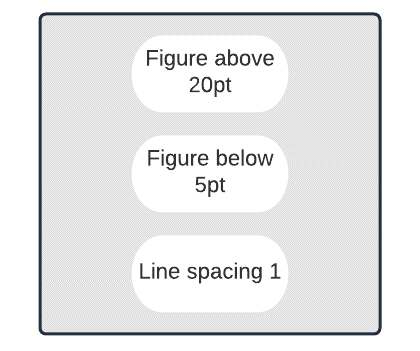
\includegraphics[scale=.8]{sample_fig.png}
\vspace{5pt}\\
\textbf{Figure 1.} Example Figure
\vspace{10pt}
\end{center}
\vspace{10pt}
{Call the figures by its sequence number in the content and give enough explanations.}
\vspace{10pt}
\section{{Results and Discussion}}
{Explain about the simulation models and simulation software. Additionally, include the comparison results with good quality pictures.}
\vspace{10pt}
\section{{Conclusion}}
{Summarize the work carried out in the proposed work.}
\vspace{10pt}
\section*{\fontsize{12}{12}\selectfont\textbf{References}}
\begin{enumerate}[{[1]}]
\item Author name1, Author name2. “Title of the paper”. Journal Name, Volume no, issue no, Page numbers. Use standard Chicago format.
\item Author name1, Author name2. “Title of the paper”. Journal Name, Volume no, issue no, Page numbers. Use standard Chicago format.
\item Author name1, Author name2. “Title of the paper”. Journal Name, Volume no, issue no, Page numbers. Use standard Chicago format.
\item Example, Duraipandian, M. "Performance evaluation of routing algorithm for Manet based on the machine learning techniques." Journal of trends in Computer Science and Smart technology (TCSST) 1, no. 01 (2019): 25-38.\\
\end{enumerate}
\vspace{10pt}
\section*{\fontsize{12}{12}\selectfont\textbf{Author's biography}}
\textbf{Author Name} Maximum of 200 words author details with photo is expected.\\
\\
\vspace{10pt}{\textbf{Second Author Name} Maximum of 200 words author details with photo is expected.}
\end{onehalfspace}
 \end{document}